\documentclass[10pt,letterpaper]{article}
% Typography adapted from the official NeurIPS 2026 author instructions.
% Course report: no conference submission, acceptance, or venue footer implied.
\usepackage[textwidth=5.5in,textheight=9in,top=1in,headheight=12pt,headsep=25pt,footskip=30pt]{geometry}
\usepackage[T1]{fontenc}
\usepackage{mathptmx}
\usepackage{microtype}
\usepackage{amsmath,amssymb}
\usepackage{booktabs,tabularx,array}
\usepackage{enumitem}
\usepackage{xcolor}
\usepackage[hidelinks]{hyperref}
\usepackage{xurl}
\usepackage[authoryear,round]{natbib}
\usepackage{caption}
\usepackage{flafter}
\usepackage{pgfplots}
\pgfplotsset{compat=1.18}
\usepgfplotslibrary{groupplots}
\definecolor{lassoblue}{HTML}{2563A6}
\definecolor{lassoorange}{HTML}{CF7A26}
\definecolor{lassogreen}{HTML}{258365}
\pgfplotsset{every axis/.append style={
  axis line style={black!55},tick style={black!45},grid style={black!10},
  title style={font=\small\bfseries},tick label style={font=\scriptsize},
  label style={font=\small},legend style={font=\scriptsize,draw=none,fill=white},
  scaled ticks=false}}
\captionsetup{font=small,labelfont=bf,labelsep=period,skip=7pt}
\captionsetup[table]{position=top,skip=7pt}
\setlength{\parskip}{5.5pt}
\setlength{\parindent}{0pt}
\setlength{\emergencystretch}{1em}
\setlength{\parfillskip}{0pt plus 1fil}
\finalhyphendemerits=10000
\hyphenation{Tibshirani Daubechies Friedman Parikh Teboulle Boyd Wright Efron}
\setlength{\textfloatsep}{14pt plus 2pt minus 2pt}
\setlength{\floatsep}{12pt plus 2pt minus 2pt}
\setlength{\intextsep}{12pt plus 2pt minus 2pt}
\renewcommand{\arraystretch}{1.12}
\renewcommand{\topfraction}{.90}
\renewcommand{\bottomfraction}{.55}
\renewcommand{\textfraction}{.08}
\renewcommand{\floatpagefraction}{.80}
\setcounter{topnumber}{3}
\setcounter{bottomnumber}{2}
\setcounter{totalnumber}{4}
\widowpenalty=10000
\clubpenalty=10000
\raggedbottom
\makeatletter
\renewcommand{\normalsize}{\@setfontsize\normalsize{10}{11}\abovedisplayskip=7pt plus2pt minus3pt\belowdisplayskip=\abovedisplayskip}
\renewcommand{\small}{\@setfontsize\small{9}{10}}
\renewcommand{\footnotesize}{\@setfontsize\footnotesize{9}{10}}
\renewcommand{\scriptsize}{\@setfontsize\scriptsize{8}{9}}
\renewcommand{\section}{\@startsection{section}{1}{\z@}{-2ex plus-.5ex minus-.2ex}{1.2ex plus.2ex}{\fontsize{12}{14}\selectfont\bfseries\raggedright}}
\renewcommand{\subsection}{\@startsection{subsection}{2}{\z@}{-1.8ex plus-.3ex minus-.2ex}{.7ex plus.2ex}{\normalsize\bfseries\raggedright}}
\makeatother
\normalsize
\newcolumntype{Y}{>{\raggedright\arraybackslash}X}
\newcommand{\R}{\mathbb{R}}
\newcommand{\soft}{\mathcal{S}}
\begin{document}
\begin{center}
\hrule height4pt
\vspace{.18in}
{\fontsize{17}{20}\selectfont\bfseries Classical Optimization Algorithms\\for Lasso Regression\par}
\vspace{5pt}
{\fontsize{11}{13}\selectfont A Review and Empirical Comparison\par}
\vspace{.14in}
\hrule height1pt
\vspace{10pt}
{\bfseries COMP6704 Group Project --- Group 9\par}
{Convex Optimization \quad | \quad 7 October 2026\par}
\vspace{9pt}
\begin{minipage}[t]{.48\linewidth}\centering\small\setlength{\parskip}{0pt}
{\normalsize\bfseries CAI Yangxiao\textsuperscript{*}}\par
The Hong Kong Polytechnic University\par
Student ID: 26023041R\par
\href{mailto:26023041r@connect.polyu.hk}{26023041r@connect.polyu.hk}
\end{minipage}\hfill
\begin{minipage}[t]{.48\linewidth}\centering\small\setlength{\parskip}{0pt}
{\normalsize\bfseries XUE Pengyu\textsuperscript{*}}\par
The Hong Kong Polytechnic University\par
Student ID: 26022951R\par
\href{mailto:26022951r@connect.polyu.hk}{26022951r@connect.polyu.hk}
\end{minipage}\par
\vspace{8pt}
\begin{minipage}[t]{.48\linewidth}\centering\small\setlength{\parskip}{0pt}
{\normalsize\bfseries ZHANG Kejia\textsuperscript{*}}\par
The Hong Kong Polytechnic University\par
Student ID: 26049131r\par
\href{mailto:26049131r@connect.polyu.hk}{26049131r@connect.polyu.hk}
\end{minipage}\hfill
\begin{minipage}[t]{.48\linewidth}\centering\small\setlength{\parskip}{0pt}
{\normalsize\bfseries ZHOU Xiyu\textsuperscript{*}}\par
The Hong Kong Polytechnic University\par
Student ID: 26025265r\par
\href{mailto:26025265r@connect.polyu.hk}{26025265r@connect.polyu.hk}
\end{minipage}
\end{center}
\begingroup
\renewcommand{\thefootnote}{\ensuremath{*}}
\footnotetext[1]{All authors contributed equally and are listed in alphabetical order by surname.}
\endgroup
\vspace{4pt}
\begin{center}\fontsize{12}{14}\selectfont\bfseries Abstract\end{center}
\begin{list}{}{\setlength{\leftmargin}{.5in}\setlength{\rightmargin}{.5in}}
\item[]
Lasso regression combines squared loss with an $\ell_1$ penalty to learn sparse linear models. We organize classical solvers by vector updates, coordinate minimization, path construction, and splitting or curvature-based steps. Basic analysis connects convexity, subgradient optimality, and soft thresholding; related penalties clarify the difference between numerical convergence and statistical selection. The empirical comparison implements ISTA, standard FISTA, and cyclic coordinate descent. Experiments on three synthetic instances and one fixed Diabetes split compare implementations under a common stationarity tolerance. All methods converge to nearly identical objectives and predictions. ISTA is fastest on the synthetic instances; coordinate descent is fastest on Diabetes. FISTA's stronger worst-case objective bound does not yield a measured time advantage under this stopping rule. Coefficient plots reveal shrinkage despite exact support recovery in the synthetic cases, while a penalty study illustrates the fit--sparsity trade-off. Results are limited to the recorded datasets, implementations, and stopping rule.
\end{list}
\vspace{3pt}
\section{Introduction}
When a regression model has many candidate predictors, a small training error can come with coefficients that are difficult to interpret. Lasso adds an $\ell_1$ penalty to the squared loss, shrinking coefficients and setting some exactly to zero \citep{tibshirani1996}. This convex linear model offers a simple setting for examining both optimization and feature selection.

The resulting objective is convex but nonsmooth at zero. Convexity excludes suboptimal local minima; it does not determine how quickly a solver reaches a useful accuracy. The comparison therefore turns on how an algorithm handles the penalty and uses the structure of the least-squares loss.

We compare ISTA, standard FISTA, and cyclic coordinate descent at the same penalty and stationarity tolerance to explain differences in convergence and computation time. A separate experiment varies the penalty to examine test error and selected variables. Keeping these comparisons separate distinguishes the effect of regularization from the cost of solving a fixed training problem.

\subsection{Scope and literature selection}
This focused narrative review concerns convex squared-loss Lasso for linear regression. It groups methods by the information used in an update and the work required to reach an accuracy target. Foundational model and solver papers are supplemented by related penalties, restarting, and safe screening. Experiments retain the three basic solvers for the same squared-loss objective.

The literature connects the three updates through a common structure (Table~\ref{tab:literature}). \citet{tibshirani1996} introduced Lasso's shrinkage and selection formulation; \citet{daubechies2004} studied iterative thresholding for inverse problems. \citet{beck2009} established the acceleration comparison, while \citet{friedman2010} developed coordinate updates for regularized regression. \citet{parikh2014} explains the proximal framework and \citet{wright2015} reviews coordinate selection rules and their assumptions. LARS supplies context on solution paths and Diabetes data \citep{efron2004}; computing an entire path is outside our fixed-penalty benchmark.

The review also separates numerical convergence from statistical selection. Uniqueness determines whether accurate solvers must agree on coefficients \citep{tibshirani2013}; support recovery needs assumptions on the predictors \citep{zhao2006}. Earlier coordinate-descent work supplies both convergence conditions \citep{tseng2001} and a regression-specific implementation \citep{wu2008}. Elastic net provides context for correlated predictors \citep{zou2005}, while the experiments retain the squared-loss Lasso objective and the same three optimization algorithms.


\begin{center}\begin{minipage}{\linewidth}\captionsetup{type=table}\centering\small
\caption{Literature organized by mechanism and question.}\label{tab:literature}
\begin{tabular*}{\linewidth}{@{\extracolsep{\fill}}lll@{}}\toprule
\textbf{Mechanism / question} & \textbf{Reference} & \textbf{Key idea}\\\midrule
Penalty geometry & \citet{tibshirani1996} & $\ell_1$\\
Thresholding & \citet{daubechies2004} & $\soft_\tau$\\
Extrapolation & \citet{beck2009} & $O(k^{-2})$\\
Scalar minimization & \citet{wu2008} & $r^{(j)}$\\
Regression paths & \citet{friedman2010} & Warm starts\\
Convergence conditions & \citet{tseng2001} & Separability\\
Coordinate choice & \citet{wright2015} & Cyclic / random\\
Curvature-based steps & \citet{kim2007} & Barrier + Newton\\
Splitting & \citet{boyd2011} & ADMM\\
Variable elimination & \citet{ndiaye2017} & Safe region\\
\bottomrule\end{tabular*}
\end{minipage}\end{center}


\section{The Lasso Training Problem}
\subsection{Objective and preprocessing}
Write $X\in\R^{n\times d}$ for the training matrix, $y\in\R^n$ for centered responses, and $w\in\R^d$ for coefficients. With $\lambda>0$ controlling regularization, the squared-loss Lasso objective is
\begin{equation}
 F(w)=g(w)+h(w)
 =\frac{1}{2n}\|Xw-y\|_2^2+\lambda\|w\|_1,\qquad\lambda>0.
 \label{eq:objective}
\end{equation}
The loss measures training fit, while the penalty encourages sparse coefficients. Every implementation uses Eq.~\eqref{eq:objective}. A different loss normalization would change both the penalty scale and the gradient, so the objective, threshold, and step size must use the same convention.

Features use their training means and population standard deviations; responses use their training mean. Test observations use the same statistics, and predictions restore the response mean. Constant training features are removed. Centering fits an unpenalized intercept without using test information.

Feature units affect coefficient magnitudes and hence the penalty. Standardization is therefore part of the model specification, and every solver receives the same transformed inputs. For comparisons with synthetic ground truth, fitted coefficients are converted back to the original feature units.

\subsection{Convex formulations}
The constrained view of Lasso minimizes the loss over a norm ball:
\begin{equation}
 \min_w g(w)\quad\text{subject to}\quad \|w\|_1\leq t,\qquad t\geq0.
 \label{eq:constrained}
\end{equation}
For any minimizer $w^\star$ of Eq.~\eqref{eq:objective}, choosing $t=\|w^\star\|_1$ makes it optimal for Eq.~\eqref{eq:constrained}. A feasible point with smaller loss would also have a smaller penalized objective. Conversely, for $t>0$, strict feasibility at $w=0$ yields a constraint multiplier $\lambda\geq0$ and a corresponding penalized problem. The correspondence need not be one-to-one \citep{tibshirani1996,boyd2004}.

Introducing $u\in\R^d$ gives an exact reformulation of the penalized model:
\begin{equation}
 \min_{w,u}\ \frac{1}{2n}\|Xw-y\|_2^2+\lambda\sum_{j=1}^d u_j
 \quad\text{subject to}\quad -u\leq w\leq u.
 \label{eq:qp}
\end{equation}
The inequalities act coordinate by coordinate. Since $\lambda>0$, every optimum has $u_j=|w_j|$. A convex quadratic objective and affine inequalities make Eq.~\eqref{eq:qp} a convex quadratic program \citep{boyd2004}. This formulation connects the norm-ball geometry with standard convex modeling; the implemented solvers work directly with the original objective in Eq.~\eqref{eq:objective}.

\subsection{Convexity, existence, and optimality}
The loss gradient supplies the fitting step in ISTA and FISTA. The Hessian is positive semidefinite because $a^\top X^\top Xa=\|Xa\|_2^2\geq0$ for every $a$, which proves convexity:
\begin{equation}
\nabla g(w)=\frac{X^\top(Xw-y)}{n},
\qquad \nabla^2g(w)=\frac{X^\top X}{n}\succeq0.
\label{eq:gradient}
\end{equation}
Hence $g$ is convex. The norm $\|w\|_1$ is also convex, so $F$ is convex. Since $\lambda>0$, $F(w)$ grows without bound as $\|w\|_2$ grows without bound; a minimizer exists. Full column rank of $X$ is a sufficient condition for strong convexity and a unique coefficient solution. Convexity alone does not guarantee uniqueness, especially in problems with more features than samples.

Full column rank is sufficient rather than necessary for uniqueness. \citet{tibshirani2013} examines unique and nonunique Lasso solutions, including problems with more predictors than observations. When coefficients are not unique, optimal solutions can have different active sets despite agreeing on fitted values. This distinction matters when using coefficient agreement to validate a solver.

The subgradient of $|u|$ at zero is $[-1,1]$. Applying this rule coordinate by coordinate gives the optimality condition below: the loss gradient must be balanced by a subgradient of the penalty.
\begin{equation}
0\in\nabla g(w^\star)+\lambda\partial\|w^\star\|_1.
\label{eq:optimality}
\end{equation}
The QP in Eq.~\eqref{eq:qp} is strictly feasible at $w=0$, $u=\mathbf{1}$, regardless of the column rank of $X$. Its Karush--Kuhn--Tucker (KKT) conditions characterize global optima and reduce to Eq.~\eqref{eq:optimality} after eliminating the auxiliary variables and multipliers \citep{boyd2004}.

The two cases are $\nabla_jg(w^\star)=-\lambda\operatorname{sign}(w_j^\star)$ for $w_j^\star\ne0$ and $|\nabla_jg(w^\star)|\leq\lambda$ for $w_j^\star=0$. The interval in the second case permits exact zeros. The same optimality condition gives a stationarity check that applies to all three solvers at a common accuracy \citep{parikh2014}.

\subsection{Why the penalty produces sparse coefficients}
Lasso and ridge both shrink coefficients: ridge uses a squared $\ell_2$ penalty, whereas Lasso uses $\ell_1$. In two dimensions, the $\ell_1$ constraint has corners on the coordinate axes, where contact with a loss contour can give a zero coefficient \citep{tibshirani1996}. The geometry explains sparsity; recovery of the generating variables still needs to be checked against known support.

Selection also depends on the feature relationships. \citet{zhao2006} links model-selection consistency to an irrepresentable condition involving the predictor covariance: sparsity alone is not enough for correct recovery. This is an asymptotic statistical result, whereas the present experiment records support on three finite synthetic instances. Convergence to a minimizer and recovery of the generating variables are separate properties and require different forms of evidence.

An orthogonal design gives a direct algebraic example. If $X^\top X/n=I$, the quadratic loss separates into scalar terms. Writing $v=X^\top y/n$, each coefficient has the following closed-form solution:
\begin{equation}
w^\star=\soft_\lambda(v),\qquad
\soft_\tau(v)_j=\operatorname{sign}(v_j)\max\{|v_j|-\tau,0\}.
\label{eq:soft}
\end{equation}
For example, $v=(1.2,-0.4,0.1)$ and $\lambda=0.3$ give $w^\star=(0.9,-0.1,0)$. The zero interval in Figure~\ref{fig:soft} removes small coefficients, while the outer segments shrink the retained ones. This analytic example explains why stronger regularization can reduce selected variables without improving test error.

The same operation appears in all three solvers. ISTA and FISTA threshold a vector after a gradient step; coordinate descent thresholds one coefficient within an exact scalar minimization. Each update follows from the objective rather than treating sparsity as a separate selection step.

\begin{center}\begin{minipage}{\linewidth}\captionsetup{type=figure}\centering
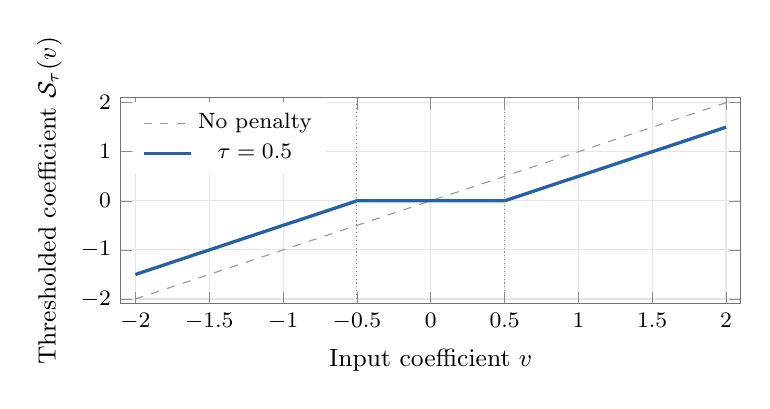
\begin{tikzpicture}
\begin{axis}[width=.78\linewidth,height=4.2cm,xmin=-2.1,xmax=2.1,ymin=-2.1,ymax=2.1,
 xlabel={Input coefficient $v$},ylabel={Thresholded coefficient $\soft_\tau(v)$},
 legend style={at={(.02,.98)},anchor=north west},grid=major]
\addplot[black!40,dashed] coordinates {(-2,-2)(2,2)};\addlegendentry{No penalty}
\addplot[lassoblue,very thick] coordinates {(-2,-1.5)(-.5,0)(.5,0)(2,1.5)};
\addlegendentry{$\tau=0.5$}
\addplot[black!45,densely dotted] coordinates {(-.5,-2)(-.5,2)};
\addplot[black!45,densely dotted] coordinates {(.5,-2)(.5,2)};
\end{axis}\end{tikzpicture}
\caption{Soft thresholding ($\tau=0.5$): zeros inside $[-\tau,\tau]$; shrinkage outside.}\label{fig:soft}
\end{minipage}\end{center}


\subsection{Related penalties: changing the model}
The same squared loss can be paired with different penalties (Table~\ref{tab:models}). Ridge adds quadratic shrinkage to stabilize estimates under nonorthogonal predictors \citep{hoerl1970}. Its smooth penalty generally retains a dense coefficient vector. Elastic net combines sparsity with quadratic shrinkage and encourages grouped selection of correlated predictors \citep{zou2005}. These choices change the estimator, even if the optimization algorithm stays the same.

\begin{center}\begin{minipage}{\linewidth}\captionsetup{type=table}\centering\small
\caption{Related convex penalties; all use the loss $g(w)$ in Eq.~\eqref{eq:objective}.}\label{tab:models}
\begin{tabular*}{\linewidth}{@{\extracolsep{\fill}}llc@{}}\toprule
\textbf{Model} & \textbf{Penalty} & \textbf{Main distinction}\\\midrule
Ridge & $\tfrac{\alpha}{2}\|w\|_2^2$ & Quadratic shrinkage\\
Lasso & $\lambda\|w\|_1$ & Uniform thresholds\\
Elastic net & $\lambda\|w\|_1+\tfrac{\alpha}{2}\|w\|_2^2$ & Grouping\\
Adaptive Lasso & $\lambda\sum_j\omega_j|w_j|$ & Weighted thresholds\\
\bottomrule\end{tabular*}
\par\vspace{3pt}{\scriptsize $\alpha,\lambda>0$; fixed $\omega_j>0$.}
\end{minipage}\end{center}

Adaptive Lasso uses weights estimated from an initial fit \citep{zou2006}. Once finite positive weights are fixed, the objective remains convex and its proximal step uses threshold $\eta\lambda\omega_j$ for coordinate $j$. The weights can distinguish coefficients that the initial fit suggests are large or small. Its statistical guarantees require assumptions on the initial estimator, design, and penalty sequence; they do not ensure that the fitted support matches the generating variables in any given finite dataset.

This comparison separates two questions. Changing a penalty asks which model gives an appropriate prediction or selection trade-off; changing a solver asks how to compute a solution to a specified objective. To isolate computation, our benchmark fixes the unweighted Lasso penalty and preprocessing before comparing the three implemented optimization algorithms.

\section{A Simple Comparison of Update Mechanisms}
Table~\ref{tab:taxonomy} compares the evaluation point, update, and dense cost per round. ISTA uses the current iterate, FISTA uses an extrapolated iterate, and coordinate descent uses the latest partial residual. A coordinate-descent round means a complete scan of all $d$ variables.


\begin{center}\begin{minipage}{\linewidth}\captionsetup{type=table}\centering\small
\caption{Update mechanisms.}\label{tab:taxonomy}
\begin{tabular*}{\linewidth}{@{\extracolsep{\fill}}lclc@{}}\toprule
\textbf{Method} & \textbf{Input} & \textbf{Update} & \textbf{Cost}\\\midrule
ISTA & $w^k$ & $\soft_{\lambda/L}(w^k-\nabla g(w^k)/L)$ & $O(nd)$\\
FISTA & $z^k$ & $\soft_{\lambda/L}(z^k-\nabla g(z^k)/L)$ & $O(nd)$\\
Cyclic CD & $r^{(j)}$ & Eq.~\eqref{eq:cd} & $O(nd)$\\
\bottomrule\end{tabular*}
\par\vspace{3pt}{\scriptsize $\eta=1/L$; CD: $d$ coordinates / sweep.}
\end{minipage}\end{center}


\subsection{ISTA}
The proximal subproblem separates across coordinates. The $\ell_1$ penalty can therefore be handled through scalar minimizations with closed-form solutions, giving the following vector operation:
\begin{equation}
\operatorname*{arg\,min}_u\left\{\frac12\|u-v\|_2^2+\tau\|u\|_1\right\}
=\soft_\tau(v).
\end{equation}
For a positive scalar solution, differentiation gives $u=v-\tau$; for a negative solution, $u=v+\tau$. If $|v|\leq\tau$, zero satisfies the subgradient condition. The three cases give soft thresholding in Eq.~\eqref{eq:soft} \citep{parikh2014}, including an interval on which the output is exactly zero.

The gradient of $g$ is Lipschitz continuous with constant $L=\|X\|_2^2/n$, where $\|X\|_2$ is the spectral norm. For $0<\eta\leq1/L$, the smooth loss has a quadratic upper bound at the current iterate. Minimizing this bound together with the penalty gives the next coefficient vector through the update
\begin{equation}
w^{k+1}=\soft_{\eta\lambda}\bigl(w^k-\eta\nabla g(w^k)\bigr).
\label{eq:ista}
\end{equation}
ISTA takes a gradient step for fitting and a thresholding step for the penalty. \citet{daubechies2004} developed iterative thresholding for linear inverse problems with sparsity constraints. Here the same mechanism solves the finite-dimensional squared-loss regression objective.

ISTA is simple to implement and has a nonincreasing objective with the stated step size. Its dense work is dominated by $Xw$ and $X^\top(Xw-y)$, without storing a full $d\times d$ matrix. Its basic objective-error bound is slower than FISTA's; choosing a smaller step can further increase the update count.

\subsection{FISTA}
FISTA applies the proximal step to an extrapolated point \citep{beck2009}. Initialize $z^1=w^0$ and $t_1=1$, then use $\eta=1/L$. The sequence $t_k$ controls the contribution of the previous direction. Each round computes the coefficients before the next extrapolation:
\begin{align}
w^k&=\soft_{\eta\lambda}\bigl(z^k-\eta\nabla g(z^k)\bigr),\\
t_{k+1}&=\frac{1+\sqrt{1+4t_k^2}}{2},\\
z^{k+1}&=w^k+\frac{t_k-1}{t_{k+1}}(w^k-w^{k-1}), \qquad k\geq1.
\end{align}
The extrapolation uses the recent direction of movement. It requires extra vector operations and a previous iterate, while the dominant matrix-vector products remain the same as those in ISTA.

For convex composite objectives with a Lipschitz-continuous smooth gradient, an existing minimizer, exact proximal updates, and step size $1/L$, the standard bounds are
\begin{align}
F(w^k)-F^\star&\leq\frac{L\|w^0-w^\star\|_2^2}{2k}
&&\text{(ISTA)},\\
F(w^k)-F^\star&\leq\frac{2L\|w^0-w^\star\|_2^2}{(k+1)^2}
&&\text{(FISTA)}.
\label{eq:rates}
\end{align}
These are objective-error bounds, not coefficient-error or elapsed-time bounds. They describe a worst-case guarantee and do not imply that every FISTA iterate improves on ISTA. Standard FISTA can have a nonmonotone objective. Our comparison uses this standard version without restart or monotonicity modifications, so that the algorithm being evaluated is unambiguous.

\subsection{Cyclic coordinate descent}
Coordinate descent fixes all coefficients except one and minimizes the resulting scalar objective. Write $x_j$ for column $j$ of $X$ and use the latest available coefficients to define

\begin{equation}
r^{(j)}=y-\sum_{\ell\ne j}x_\ell w_\ell.
\end{equation}
The scalar objective contains a quadratic loss and an absolute-value penalty. Its solution uses soft thresholding, divided by the squared norm of the feature column to account for its scale:
\begin{equation}
\begin{gathered}
\min_u\frac{1}{2n}\|r^{(j)}-x_ju\|_2^2+\lambda|u|,\\
w_j\leftarrow
\frac{\soft_\lambda(x_j^\top r^{(j)}/n)}{\|x_j\|_2^2/n}.
\end{gathered}
\label{eq:cd}
\end{equation}
The denominator is one for centered, unit-variance columns. The general formula retains the dependence on feature scaling, as in the regression coordinate update of \citet{friedman2010}.

Maintain $r=y-Xw$ throughout the sweep. Before updating coordinate $j$, form $r^{(j)}=r+x_jw_j$; afterwards, set $r=r^{(j)}-x_jw_j$. Each coordinate costs $O(n)$ for dense data, and a sweep costs $O(nd)$. Updating the residual after every coefficient change avoids repeated full predictions.

\citet{wu2008} studies cyclic coordinate descent for squared-error regression with a Lasso penalty. That setting matches our scalar updates; the paper's absolute-error and grouped extensions are outside this report. It provides a second regression-specific source alongside the pathwise implementation of \citet{friedman2010} for regularized least-squares regression.


{
Exact coordinate minimization makes the objective nonincreasing and needs no global gradient step size. Update order and problem assumptions still matter. \citet{wright2015} distinguishes cyclic, randomized, smooth, and regularized methods. A randomized rate cannot be transferred directly to this cyclic Lasso implementation; the rate entry is therefore left unspecified.\par}

\citet{tseng2001} analyzes block coordinate descent when the nonsmooth component is separable and further regularity conditions hold. In Lasso, $\|w\|_1=\sum_j|w_j|$ supplies this separability. The result explains why the structure of the penalty matters; it does not justify convergence claims for arbitrary nonsmooth objectives or an unconditional rate for our implementation.


\section{The Wider Solver Landscape}
The three implemented methods use either a full vector or one coordinate at a time. Other approaches use a solution path, curvature information, or an equality-constrained split. Table~\ref{tab:families} compares their operations and additional work; their iteration counts refer to different optimization subproblems.

\begin{center}\begin{minipage}{\linewidth}\captionsetup{type=table}\centering\small
\caption{Solver families and the work they expose.}\label{tab:families}
\begin{tabular*}{\linewidth}{@{\extracolsep{\fill}}lll@{}}\toprule
\textbf{Family} & \textbf{Main operation} & \textbf{Extra work / state}\\\midrule
ISTA / FISTA & Vector threshold & Matrix-vector products\\
Coordinate descent & Scalar minimization & Residual; coordinate scan\\
LARS--Lasso & Path segment & Active-set linear algebra\\
Interior point & Barrier Newton step & Linear-system iterations\\
ADMM & Split subproblems & Linear solve; dual state\\
\bottomrule\end{tabular*}
\end{minipage}\end{center}

\subsection{Paths, curvature, and splitting}
LARS with the Lasso modification follows the solution path as the penalty changes \citep{efron2004}. Pathwise coordinate descent instead solves successive penalties with warm starts \citep{friedman2010}. Reusing a nearby solution can reduce subsequent work, but path construction and a cold solve at one penalty have different costs. Our fixed-penalty runs start at zero; the separate penalty study is not a benchmark of either of these methods for constructing solution paths.

\citet{kim2007} introduces auxiliary bounds on coefficients to express the absolute-value penalty as a linear term in a quadratic program. A logarithmic barrier gives approximate Newton steps, computed with preconditioned conjugate gradients in their specialized implementation. This replaces many simple updates with more involved linear algebra. Its value depends on structure and accuracy; paper timings do not describe the runtime of a generic quadratic-program solver.

ADMM separates the quadratic loss and the $\ell_1$ penalty using an equality constraint \citep{boyd2011}. Its Lasso iteration alternates a regularized linear solve, soft thresholding, and a dual update. The algorithmic penalty is distinct from the model's $\lambda$; fixing it can permit factorization reuse. Consequently, setup and solve costs both matter when comparing this splitting method with the matrix-vector operations used by the two proximal-gradient implementations in this report.

\subsection{Reducing repeated or unnecessary work}
Acceleration can create oscillations, so momentum management is a separate design choice. \citet{odonoghue2015} proposes restarting based on objective or gradient criteria and discusses a FISTA application. Resetting extrapolation may help when its direction is unproductive, but frequent restarting can also slow progress. The paper suggests an extension to standard FISTA; residual oscillations do not establish that restarting would reduce our measured runtime.

Safe screening removes variables only when a valid test proves that their optimal coefficients are zero \citep{ndiaye2017}. Gap Safe rules form a region containing the dual optimum from a dual-feasible point and a primal--dual gap. A shrinking region can exclude more variables as optimization progresses. Screening adds certificate calculations but reduces the optimization dimension; its usefulness depends on the feature count and the amount of work that can be removed.

The gap is also an accuracy certificate: a primal objective minus a feasible dual lower bound bounds objective suboptimality. This differs from our stationarity-residual threshold. Neither criterion identifies the generating variables merely by certifying optimization progress. The broader literature therefore suggests three distinct comparisons: update mechanisms, reusable or removable work, and the certificate used to declare a solution accurate enough for the stated training problem.

\section{Strengths, Weaknesses, and Comparison Limits}
Table~\ref{tab:tradeoffs} records monotonicity and objective-error bounds. ISTA and FISTA assume a convex objective, a Lipschitz-continuous smooth gradient, exact proximal updates, and a valid step size \citep{beck2009}. No universal rate is assigned to cyclic coordinate descent.


\begin{center}\begin{minipage}{\linewidth}\captionsetup{type=table}\centering\small
\caption{Monotonicity and objective-error bounds.}\label{tab:tradeoffs}
\begin{tabular*}{\linewidth}{@{\extracolsep{\fill}}lcccc@{}}\toprule
\textbf{Method} & $\mathbf{F_{k+1}\leq F_k}$ & \textbf{Bound} & \textbf{Step} & \textbf{State}\\\midrule
ISTA & $\checkmark$ & $O(k^{-1})$ & $1/L$ & ---\\
FISTA & --- & $O(k^{-2})$ & $1/L$ & $z,t$\\
Cyclic CD & $\checkmark$ & --- & --- & $r$\\
\bottomrule\end{tabular*}
\par\vspace{3pt}{\scriptsize $F_k=F(w^k)$; $\checkmark$: monotone; ---: no claim / n.a.}
\end{minipage}\end{center}


A scalar coordinate update is smaller than a vector update, so we compare complete CD sweeps with ISTA/FISTA rounds and also report time. Dense work is $O(nd)$ per round, but loops and matrix-vector kernels have different overheads. Accurate solvers at a fixed penalty should reach similar objectives; coefficient agreement additionally depends on uniqueness.

The penalty controls the fit--sparsity trade-off. A test-error difference at a fixed penalty should first be checked against stopping accuracy and preprocessing. Changing the penalty studies the model rather than the solver, and a sparse fit alone does not establish recovery of the generating variables.

\section{Data and Experimental Protocol}
\subsection{Data}
All experiments read the saved inputs and fixed splits in Table~\ref{tab:data}. Features and responses retain their original units, and each observation has a recorded split assignment. Centering and scaling use only the selected training rows, so all solvers receive identical transformed data.


\begin{center}\begin{minipage}{\linewidth}\captionsetup{type=table}\centering\small
\caption{Dataset sizes per instance.}\label{tab:data}
\begin{tabular*}{\linewidth}{@{\extracolsep{\fill}}lrrrr@{}}\toprule
\textbf{Input} & \textbf{Instances} & \textbf{$N$} & \textbf{$d$} & \textbf{Train / test}\\\midrule
Synthetic sparse regression & 3 & 300 & 50 & 240 / 60\\
Diabetes regression & 1 & 442 & 10 & 353 / 89\\
\bottomrule\end{tabular*}\end{minipage}\end{center}


Synthetic features are independent standard-normal draws. The first five true coefficients are $(2,-1.5,1,-2,1.5)$, and the remaining 45 are zero. Responses satisfy $y=Xw_{\mathrm{true}}+\varepsilon$ with normal noise of standard deviation 0.5. Seeds 0, 1, and 2 define three independently generated instances.

Diabetes contains 442 observations, ten baseline predictors, and a continuous measure of disease progression one year later \citep{efron2004}. We use the raw files distributed with scikit-learn 1.9.1 and standardize them on the training split \citep{sklearn_data}. Unlike the synthetic instances, this dataset has no known generating coefficients or correct support set.

A separate NumPy generator permutes row indices with the recorded split seed. The first $\lceil0.2N\rceil$ rows form the test set. Split seeds are 0, 1, and 2 for the synthetic instances and zero for Diabetes. Saved split assignments and input hashes identify the observations used in the experiments.

\subsection{Common settings and stopping check}
{
Table~\ref{tab:settings} gives the settings fixed before measurement. The penalty scale comes from the transformed training inputs. A zero vector becomes optimal at the largest absolute feature--response inner product divided by sample size. This defines the training-dependent reference value\par}
\begin{equation}
\lambda_{\max}=\frac{\|X^\top y\|_\infty}{n}.
\end{equation}
Eq.~\eqref{eq:optimality} shows that $w=0$ is optimal when $\lambda\geq\lambda_{\max}$. The main comparison uses $\lambda=0.1\lambda_{\max}$. This choice provides a nontrivial sparse fit; it is not claimed to minimize prediction error.


\begin{center}\begin{minipage}{\linewidth}\captionsetup{type=table}\centering\small
\caption{Experimental settings.}\label{tab:settings}
\begin{tabular*}{\linewidth}{@{\extracolsep{\fill}}ll@{}}\toprule
\textbf{Setting} & \textbf{Value}\\\midrule
Initialization & $w^0=0$\\
Penalty & $\lambda/\lambda_{\max}=0.1$\\
ISTA / FISTA step & $\eta=1/L,\quad L=\|X\|_2^2/n$\\
CD order & $j=1,\ldots,d$\\
Stopping & $R\leq10^{-6}$\\
Maximum rounds & $10^4$\\
Timing & $5$ repeats; median\\
Penalty ratios & $\{0.01,\,0.1,\,0.5,\,1\}$ (CD)\\
\bottomrule\end{tabular*}
\end{minipage}\end{center}


A common stopping check is needed because small parameter changes do not necessarily imply comparable optimization accuracy. Define the proximal-gradient mapping and normalized residual
\begin{align}
G_L(w)&=L\left[w-\soft_{\lambda/L}
                  \left(w-\frac{\nabla g(w)}{L}\right)\right],\\
R(w)&=\frac{\|G_L(w)\|_\infty}
{\max\{1,\|X^\top y/n\|_\infty\}}.
\label{eq:residual}
\end{align}
The mapping is zero exactly when the optimality condition holds \citep{parikh2014}. Its norm measures stationarity; it does not certify an upper bound on objective error. We evaluate it after every vector update or CD sweep, at the returned coefficient vector rather than the FISTA extrapolation point. A run that reaches its iteration limit before meeting the threshold is marked as unconverged.

\subsection{Comparison and measurement}
At a fixed penalty, we compare objective trajectories, stationarity residuals, complete rounds, and elapsed time. Test MSE and nonzero counts describe the resulting fit. They answer a different question from the computation required to reach the prescribed optimization tolerance.

Timing includes algorithm-specific preparation, objective recording, and the common residual check. Loading, preprocessing, the shared spectral-norm calculation, and plotting are excluded. No solver uses a precomputed Gram matrix or screening. Five timing repetitions yield one median per instance; the synthetic summary reports variation over three instances, while Diabetes uses one fixed split.

For the penalty study, CD solves four prespecified values to the same tolerance. We report test MSE and coefficients satisfying $|w_j|>10^{-6}$ in standardized units. The test scores describe these settings; they are not used to select a penalty and then claim an unbiased estimate of its prediction error.

\subsection{Minimal implementation validation}
We first check an orthogonal design against Eq.~\eqref{eq:soft}, then compare synthetic seed 0 with a tighter scikit-learn solve. The reference uses centered inputs, $\texttt{alpha}=\lambda$, and no fitted intercept, matching the documented objective \citep{sklearn_data}. Comparing coefficients, objective, and stationarity residual checks numerical agreement before the timed runs.

The orthogonal case checks thresholding and normalization against a closed-form solution. The reference case checks a nonorthogonal design against another implementation. Both checks precede the timed runs and address numerical correctness rather than providing evidence about solver speed.

\section{Experimental Results and Discussion}
\subsection{Validation and execution}
Both implementation checks passed. The largest absolute coefficient error on the orthogonal instance was $1.12\times10^{-15}$. On synthetic seed 0, relative objective differences from the tighter scikit-learn reference were at most $1.57\times10^{-12}$; the reference residual was $1.54\times10^{-14}$. These checks support the implemented normalization and updates, but do not certify a general solver ranking.

All 60 main timing runs (four instances, three methods, five repetitions) and all 16 regularization runs reached $R\leq10^{-6}$. Execution used Python 3.12.14, NumPy 2.3.5, scikit-learn 1.9.1, and Matplotlib 3.11.2 on an arm64 macOS host, with available numerical thread pools limited to one thread. Raw timings, histories, coefficients, input hashes, and environment versions are retained.

\subsection{Efficiency at a common tolerance}


\begin{center}\begin{minipage}{\linewidth}\captionsetup{type=table}\centering\small
\caption{Solver comparison at $\lambda/\lambda_{\max}=0.1$.}\label{tab:optimization_results}
\begin{tabular*}{\linewidth}{@{\extracolsep{\fill}}lrrrr@{}}\toprule
\textbf{Method} & \textbf{Time (ms)} & \textbf{Rounds} & \textbf{Final $F$} & \textbf{$R$ ($10^{-6}$)}\\\midrule
\multicolumn{5}{@{}l}{\textit{Synthetic: three instances}}\\[2pt]
ISTA & $\mathbf{0.389}\,{\pm}\,0.013$ & $24.7\,{\pm}\,0.6$ & $1.800\,{\pm}\,0.174$ & $0.71\,{\pm}\,0.16$\\
FISTA & $0.519\,{\pm}\,0.035$ & $30.7\,{\pm}\,2.3$ & $1.800\,{\pm}\,0.174$ & $0.53\,{\pm}\,0.30$\\
CD & $0.596\,{\pm}\,0.010$ & $5.0$ & $1.800\,{\pm}\,0.174$ & $0.14\,{\pm}\,0.17$\\
\midrule
\multicolumn{5}{@{}l}{\textit{Diabetes: fixed split}}\\[2pt]
ISTA & $1.419$ & $92.0$ & $1812.178$ & $0.99$\\
FISTA & $1.437$ & $85.0$ & $1812.178$ & $0.31$\\
CD & $\mathbf{0.530}$ & $14.0$ & $1812.178$ & $0.40$\\
\bottomrule\end{tabular*}\par\vspace{3pt}{\scriptsize $\mu\pm s$: three instances; $t=\mathrm{median}(5)$; \textbf{bold}: min. $t$.}\end{minipage}\end{center}


On the synthetic instances, ISTA used 24--25 updates, FISTA used 28--32, and CD used five sweeps. ISTA had the shortest measured time on all three instances. CD completed fewer sweeps but each sweep made 50 sequential scalar updates in a Python loop. ISTA and FISTA used NumPy matrix-vector operations. These timings are consistent with loop overhead affecting CD at this size, although loop overhead was not measured by timing the individual operations separately.

On Diabetes, CD required 14 sweeps and a median of 0.530 ms, compared with 92 updates and 1.419 ms for ISTA and 85 updates and 1.437 ms for FISTA. CD was fastest in this setting. ISTA and FISTA timing ranges overlapped: 1.326--1.438 ms and 1.357--1.450 ms, respectively. Their small median difference does not support a robust speed distinction between these vector methods.

\begin{center}\begin{minipage}{\linewidth}\captionsetup{type=figure}\centering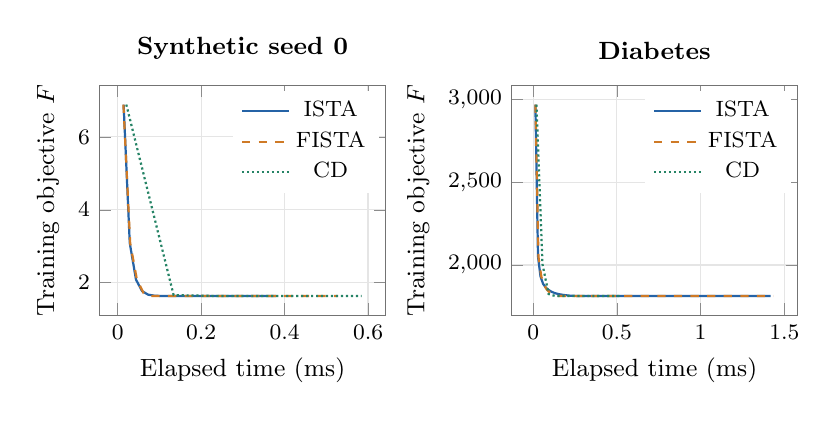
\begin{tikzpicture}
\begin{groupplot}[group style={group size=2 by 1,horizontal sep=1.6cm},width=.43\linewidth,height=4.5cm,
xlabel={Elapsed time (ms)},ylabel={Training objective $F$},tick label style={font=\scriptsize},label style={font=\small},
legend style={font=\scriptsize,at={(.98,.98)},anchor=north east},grid=major]
\nextgroupplot[title={Synthetic seed 0}]
\addplot[lassoblue,thick] coordinates {(0.014042,6.88816286) (0.02875,3.08833414) (0.043708,2.08334595) (0.058333,1.76622752) (0.072917,1.66970236) (0.08775,1.64264139) (0.102208,1.63474449) (0.11675,1.63240592) (0.131458,1.63170413) (0.145875,1.63149098) (0.160625,1.63142551) (0.175167,1.6314052) (0.19,1.63139884) (0.204458,1.63139683) (0.219208,1.63139618) (0.23375,1.63139598) (0.248292,1.63139591) (0.262875,1.63139589) (0.277417,1.63139588) (0.29175,1.63139588) (0.30625,1.63139588) (0.32075,1.63139588) (0.335125,1.63139588) (0.349833,1.63139588) (0.364167,1.63139588) (0.378958,1.63139588)};
\addlegendentry{ISTA}
\addplot[lassoorange,thick,dashed] coordinates {(0.013541,6.88816286) (0.02975,3.08833414) (0.045833,2.08334595) (0.061958,1.7112345) (0.078541,1.63547811) (0.094625,1.63244396) (0.111,1.63336655) (0.126916,1.63227743) (0.143083,1.63153593) (0.159375,1.6314073) (0.175333,1.6314265) (0.191666,1.63141931) (0.207541,1.63140285) (0.223708,1.63139667) (0.239791,1.63139653) (0.255708,1.63139667) (0.271833,1.63139626) (0.287708,1.63139596) (0.303666,1.6313959) (0.318791,1.63139591) (0.3345,1.6313959) (0.3505,1.63139589) (0.366458,1.63139588) (0.382625,1.63139588) (0.398416,1.63139588) (0.414791,1.63139588) (0.430875,1.63139588) (0.447041,1.63139588) (0.463083,1.63139588) (0.478916,1.63139588) (0.495125,1.63139588) (0.511083,1.63139588) (0.527208,1.63139588)};
\addlegendentry{FISTA}
\addplot[lassogreen,thick,densely dotted] coordinates {(0.0205,6.88816286) (0.133875,1.65801906) (0.247292,1.63145421) (0.360208,1.63139596) (0.4725,1.63139588) (0.584917,1.63139588)};
\addlegendentry{CD}
\nextgroupplot[title={Diabetes}]
\addplot[lassoblue,thick] coordinates {(0.013375,2969.82747) (0.029,2050.30114) (0.043959,1930.58044) (0.059084,1886.46583) (0.0745,1864.78393) (0.089917,1850.6147) (0.105417,1840.81119) (0.120167,1833.73688) (0.135459,1828.42813) (0.151167,1824.29919) (0.168542,1821.05043) (0.18475,1818.47128) (0.203,1816.3806) (0.218875,1814.66252) (0.234417,1813.86647) (0.249834,1813.3972) (0.264375,1813.07135) (0.279875,1812.83782) (0.295,1812.66842) (0.3105,1812.54449) (0.325209,1812.45314) (0.340625,1812.38535) (0.356,1812.33472) (0.371334,1812.29668) (0.385875,1812.26795) (0.401209,1812.24615) (0.416792,1812.22954) (0.432459,1812.21683) (0.446875,1812.20706) (0.462125,1812.19954) (0.477084,1812.19373) (0.492125,1812.18923) (0.507542,1812.18574) (0.52275,1812.18321) (0.538167,1812.18191) (0.553584,1812.18096) (0.569084,1812.18022) (0.584625,1812.17965) (0.599459,1812.1792) (0.61475,1812.17885) (0.629334,1812.17857) (0.643542,1812.17835) (0.658875,1812.17818) (0.673709,1812.17804) (0.68825,1812.17793) (0.703834,1812.17784) (0.719167,1812.17778) (0.734334,1812.17772) (0.748959,1812.17768) (0.764167,1812.17765) (0.778959,1812.17762) (0.79375,1812.1776) (0.809084,1812.17758) (0.824459,1812.17757) (0.840125,1812.17756) (0.854709,1812.17755) (0.87,1812.17754) (0.885375,1812.17754) (0.90075,1812.17753) (0.915459,1812.17753) (0.930709,1812.17753) (0.945584,1812.17752) (0.960125,1812.17752) (0.97525,1812.17752) (0.990792,1812.17752) (1.006209,1812.17752) (1.020917,1812.17752) (1.036459,1812.17752) (1.05175,1812.17752) (1.067042,1812.17752) (1.081875,1812.17752) (1.097292,1812.17752) (1.112167,1812.17752) (1.127417,1812.17752) (1.142917,1812.17752) (1.157834,1812.17752) (1.173459,1812.17752) (1.189292,1812.17752) (1.204542,1812.17752) (1.219917,1812.17752) (1.234709,1812.17752) (1.25025,1812.17752) (1.265625,1812.17752) (1.28125,1812.17752) (1.29575,1812.17752) (1.311209,1812.17752) (1.326917,1812.17752) (1.342292,1812.17752) (1.356917,1812.17752) (1.3725,1812.17752) (1.38825,1812.17752) (1.403709,1812.17752) (1.418417,1812.17752)};
\addlegendentry{ISTA}
\addplot[lassoorange,thick,dashed] coordinates {(0.01375,2969.82747) (0.0315,2050.30114) (0.048709,1930.58044) (0.065375,1877.93191) (0.082209,1850.5917) (0.098792,1833.75095) (0.115542,1823.4414) (0.1325,1816.67353) (0.149,1813.16557) (0.166,1812.49494) (0.182209,1812.44568) (0.198625,1812.35462) (0.215084,1812.27607) (0.231542,1812.25221) (0.248459,1812.23365) (0.264709,1812.21414) (0.281625,1812.20067) (0.2985,1812.19301) (0.315084,1812.18785) (0.332084,1812.18383) (0.348667,1812.18104) (0.3655,1812.17972) (0.382417,1812.17966) (0.399,1812.18014) (0.415709,1812.18041) (0.432625,1812.18009) (0.449459,1812.1793) (0.466375,1812.17841) (0.483042,1812.17778) (0.499584,1812.17753) (0.516875,1812.17759) (0.533584,1812.17776) (0.550375,1812.17789) (0.567084,1812.17792) (0.584042,1812.17785) (0.600542,1812.17773) (0.617167,1812.17762) (0.634209,1812.17755) (0.651,1812.17752) (0.667667,1812.17753) (0.684792,1812.17755) (0.7015,1812.17757) (0.718584,1812.17757) (0.735084,1812.17757) (0.751959,1812.17755) (0.768584,1812.17754) (0.785459,1812.17753) (0.802292,1812.17752) (0.818667,1812.17752) (0.835792,1812.17752) (0.852292,1812.17752) (0.869125,1812.17753) (0.886209,1812.17753) (0.902834,1812.17753) (0.919834,1812.17752) (0.936459,1812.17752) (0.95325,1812.17752) (0.970209,1812.17752) (0.986917,1812.17752) (1.003542,1812.17752) (1.020167,1812.17752) (1.037084,1812.17752) (1.053959,1812.17752) (1.070292,1812.17752) (1.086834,1812.17752) (1.103584,1812.17752) (1.120084,1812.17752) (1.137042,1812.17752) (1.153709,1812.17752) (1.1705,1812.17752) (1.186917,1812.17752) (1.203875,1812.17752) (1.220625,1812.17752) (1.237084,1812.17752) (1.253917,1812.17752) (1.270209,1812.17752) (1.286917,1812.17752) (1.304167,1812.17752) (1.320792,1812.17752) (1.337584,1812.17752) (1.353917,1812.17752) (1.370584,1812.17752) (1.387334,1812.17752) (1.403709,1812.17752) (1.42075,1812.17752) (1.436875,1812.17752)};
\addlegendentry{FISTA}
\addplot[lassogreen,thick,densely dotted] coordinates {(0.019666,2969.82747) (0.055708,2005.32301) (0.092,1824.81235) (0.1285,1813.4361) (0.164666,1812.45249) (0.200875,1812.23124) (0.237625,1812.18465) (0.27425,1812.17817) (0.310291,1812.17756) (0.346958,1812.17752) (0.383166,1812.17752) (0.42025,1812.17752) (0.456875,1812.17752) (0.493833,1812.17752) (0.529833,1812.17752)};
\addlegendentry{CD}
\end{groupplot}\end{tikzpicture}
\caption{Objective versus time; median-time repetition.}\label{fig:objective}\end{minipage}\end{center}

\begin{center}\begin{minipage}{\linewidth}\captionsetup{type=figure}\centering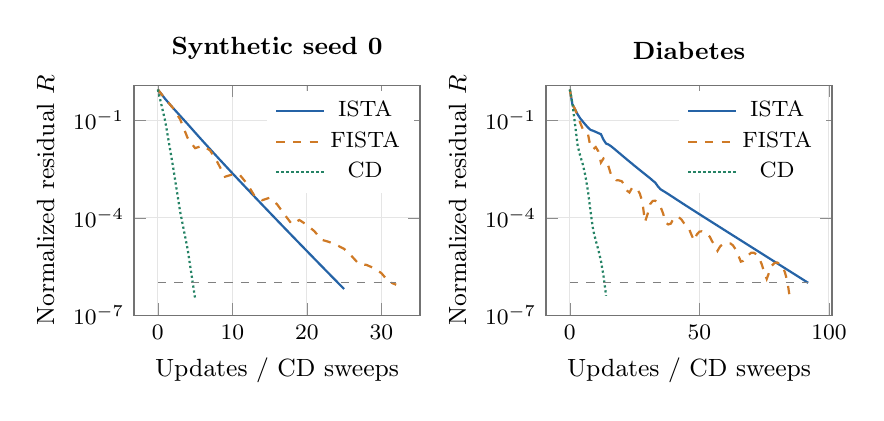
\begin{tikzpicture}
\begin{groupplot}[group style={group size=2 by 1,horizontal sep=1.6cm},width=.43\linewidth,height=4.5cm,
xlabel={Updates / CD sweeps},ylabel={Normalized residual $R$},tick label style={font=\scriptsize},label style={font=\small},
legend style={font=\scriptsize,at={(.98,.98)},anchor=north east},grid=major,ymode=log,ymin=1e-7,ymax=1.2]
\nextgroupplot[title={Synthetic seed 0}]
\addplot[lassoblue,thick] coordinates {(0,0.9) (1,0.455432794) (2,0.247670845) (3,0.138544221) (4,0.0773012068) (5,0.0425593593) (6,0.0236163258) (7,0.013194505) (8,0.00741544914) (9,0.00418884594) (10,0.00237662974) (11,0.00135357471) (12,0.000773465739) (13,0.000443260214) (14,0.000254675294) (15,0.000146657014) (16,8.46264203e-05) (17,4.89230007e-05) (18,2.83305828e-05) (19,1.64314636e-05) (20,9.54394086e-06) (21,5.55098381e-06) (22,3.2327263e-06) (23,1.88493123e-06) (24,1.10033356e-06) (25,6.43032941e-07)};
\addlegendentry{ISTA}
\addplot[lassoorange,thick,dashed] coordinates {(0,0.9) (1,0.455432794) (2,0.247670845) (3,0.107287112) (4,0.0286748138) (5,0.013988644) (6,0.0166127806) (7,0.0120377777) (8,0.00517466003) (9,0.00184270731) (10,0.00216520401) (11,0.00210331947) (12,0.00110672139) (13,0.000466002569) (14,0.000347819375) (15,0.000414355258) (16,0.000262697346) (17,0.00012704316) (18,6.36685352e-05) (19,8.57895853e-05) (20,6.06191939e-05) (21,3.91170211e-05) (22,2.11303593e-05) (23,1.80524117e-05) (24,1.45516654e-05) (25,1.10728532e-05) (26,6.70073133e-06) (27,3.75921441e-06) (28,3.55788106e-06) (29,2.82997587e-06) (30,1.98910065e-06) (31,1.081225e-06) (32,8.68686252e-07)};
\addlegendentry{FISTA}
\addplot[lassogreen,thick,densely dotted] coordinates {(0,0.9) (1,0.0930033112) (2,0.00424004028) (3,0.000151798178) (4,1.07123657e-05) (5,3.29790039e-07)};
\addlegendentry{CD}
\addplot[gray,dashed] coordinates {(0,1e-6)(32.0,1e-6)};
\nextgroupplot[title={Diabetes}]
\addplot[lassoblue,thick] coordinates {(0,0.9) (1,0.312844631) (2,0.222650828) (3,0.154780351) (4,0.116053875) (5,0.0923689123) (6,0.0745748373) (7,0.0605940121) (8,0.0511568099) (9,0.0481669247) (10,0.0443499139) (11,0.0407596221) (12,0.0379082544) (13,0.0254382722) (14,0.0194158551) (15,0.0179883867) (16,0.0158165098) (17,0.0136521792) (18,0.0117092801) (19,0.0100253969) (20,0.00858399326) (21,0.00735502818) (22,0.00630793048) (23,0.00541530384) (24,0.0046536038) (25,0.00400289048) (26,0.00344635359) (27,0.00296983055) (28,0.00256137938) (29,0.00221091653) (30,0.00190991454) (31,0.00165115069) (32,0.0014037249) (33,0.00120539424) (34,0.000931642495) (35,0.000758806932) (36,0.000677457246) (37,0.000606322474) (38,0.00053929133) (39,0.000478487984) (40,0.00042423346) (41,0.000376154421) (42,0.000333652941) (43,0.000296098395) (44,0.000262900007) (45,0.00023352928) (46,0.00020752229) (47,0.000184474616) (48,0.000164034215) (49,0.000145894313) (50,0.000129787016) (51,0.000115477817) (52,0.000102760951) (53,9.14554685e-05) (54,8.14019404e-05) (55,7.2459659e-05) (56,6.45042615e-05) (57,5.74256962e-05) (58,5.11264758e-05) (59,4.55201677e-05) (60,4.05300851e-05) (61,3.60881466e-05) (62,3.21338803e-05) (63,2.86135505e-05) (64,2.54793908e-05) (65,2.26889284e-05) (66,2.02043885e-05) (67,1.7992168e-05) (68,1.60223695e-05) (69,1.42683892e-05) (70,1.27065512e-05) (71,1.13157835e-05) (72,1.00773296e-05) (73,8.97449338e-06) (74,7.99241179e-06) (75,7.1178529e-06) (76,6.3390365e-06) (77,5.64547439e-06) (78,5.02782846e-06) (79,4.47778431e-06) (80,3.98793891e-06) (81,3.5517005e-06) (82,3.16319965e-06) (83,2.81720999e-06) (84,2.50907767e-06) (85,2.23465865e-06) (86,1.99026273e-06) (87,1.77260387e-06) (88,1.57875586e-06) (89,1.40611292e-06) (90,1.25235457e-06) (91,1.11541436e-06) (92,9.9345208e-07)};
\addlegendentry{ISTA}
\addplot[lassoorange,thick,dashed] coordinates {(0,0.9) (1,0.312844631) (2,0.222650828) (3,0.13604825) (4,0.0854274238) (5,0.0540496603) (6,0.0431792404) (7,0.0380406496) (8,0.0148292564) (9,0.0129669057) (10,0.0151378103) (11,0.0111515318) (12,0.0050608895) (13,0.0067431841) (14,0.00579191077) (15,0.00367275051) (16,0.00200573574) (17,0.00179423963) (18,0.00144324851) (19,0.00142309985) (20,0.00134502114) (21,0.00105895738) (22,0.000696115654) (23,0.000602771851) (24,0.000830771642) (25,0.000875049425) (26,0.000767574817) (27,0.000560963147) (28,0.000311929386) (29,7.53418206e-05) (30,0.000129044606) (31,0.00026476) (32,0.000331788757) (33,0.000336640796) (34,0.000293684136) (35,0.000220841131) (36,0.000135826334) (37,7.14098962e-05) (38,6.2395776e-05) (39,6.64911337e-05) (40,9.67707025e-05) (41,0.000108334938) (42,0.000104721915) (43,9.03217949e-05) (44,6.95251322e-05) (45,5.77670008e-05) (46,4.61016881e-05) (47,2.93377798e-05) (48,1.97294214e-05) (49,3.05521857e-05) (50,3.75006312e-05) (51,3.85707228e-05) (52,3.50875129e-05) (53,3.1542831e-05) (54,2.62341786e-05) (55,1.8444674e-05) (56,1.40556446e-05) (57,9.60896146e-06) (58,1.31146818e-05) (59,1.53480857e-05) (60,1.53426486e-05) (61,1.67752404e-05) (62,1.62466069e-05) (63,1.40504817e-05) (64,1.06262972e-05) (65,7.05070175e-06) (66,4.47358841e-06) (67,4.74525363e-06) (68,5.53942917e-06) (69,7.24506371e-06) (70,8.37745355e-06) (71,8.41892983e-06) (72,7.51274995e-06) (73,5.89103407e-06) (74,3.83594558e-06) (75,2.17187394e-06) (76,1.31275347e-06) (77,2.15538817e-06) (78,3.39426179e-06) (79,4.07629939e-06) (80,4.20555847e-06) (81,3.84792564e-06) (82,3.11436048e-06) (83,2.14152063e-06) (84,1.07244817e-06) (85,3.06545108e-07)};
\addlegendentry{FISTA}
\addplot[lassogreen,thick,densely dotted] coordinates {(0,0.9) (1,0.327877931) (2,0.0775597041) (3,0.0170256008) (4,0.00817497355) (5,0.00445160408) (6,0.00197713935) (7,0.000662787183) (8,0.000156902603) (9,4.21225636e-05) (10,1.99724439e-05) (11,1.0396302e-05) (12,4.73637475e-06) (13,1.62027709e-06) (14,3.96129418e-07)};
\addlegendentry{CD}
\addplot[gray,dashed] coordinates {(0,1e-6)(92.0,1e-6)};
\end{groupplot}\end{tikzpicture}
\caption{Residual versus rounds. Dashed line: $R=10^{-6}$.}\label{fig:stationarity}\end{minipage}\end{center}

{
Figure~\ref{fig:stationarity} shows oscillations in FISTA's residual and a smoother decrease for ISTA. Acceleration did not reduce the synthetic update count at this threshold. Eq.~\eqref{eq:rates} bounds worst-case objective error, whereas the stopping rule concerns an instance's proximal-gradient residual. Initial objective reduction alone therefore cannot determine time to the declared tolerance (Figure~\ref{fig:objective}). These observations concern standard FISTA; restart variants need a separate comparison.\par}

The shared spectral-norm calculation took 0.278--0.714 ms for synthetic instances and 3.070 ms for Diabetes. It is excluded from Table~\ref{tab:optimization_results} but would matter in an end-to-end application at these sizes. CD does not need $L$ for its scalar update; the common residual check does. These timings depend on the recorded input sizes, the solver and monitoring implementations, and the machine.


\subsection{What the timing repetitions establish}
Figure~\ref{fig:timing} retains all five measurements rather than displaying only medians. ISTA's range lies below the other methods' ranges on each synthetic instance, while CD's range lies below both vector methods on Diabetes. The ISTA/FISTA overlap on Diabetes supports treating their small median difference cautiously. No significance test is claimed from five short timing repetitions.

Rounds and time give different rankings. Five synthetic CD sweeps contain $5\times50=250$ scalar updates; a 25-round ISTA run contains 25 vector updates. Both have dense work of order $nd$ per round, but scalar loops and matrix-vector kernels differ. This is consistent with an implementation cost explanation, although the experiment does not isolate the overhead of each operation.

\begin{center}\begin{minipage}{\linewidth}\captionsetup{type=figure}\centering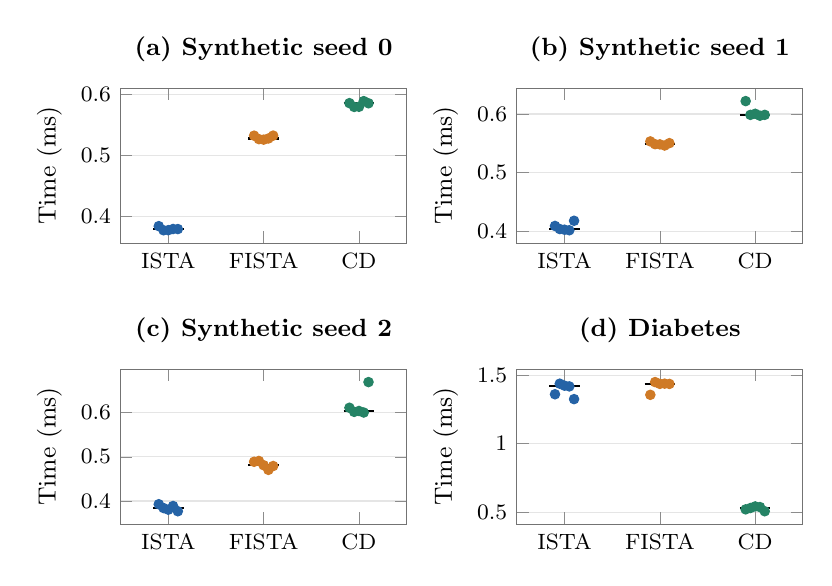
\begin{tikzpicture}
\begin{groupplot}[group style={group size=2 by 2,horizontal sep=1.4cm,vertical sep=1.6cm},
width=.43\linewidth,height=3.55cm,xmin=.5,xmax=3.5,xtick={1,2,3},xticklabels={ISTA,FISTA,CD},ylabel={Time (ms)},ymajorgrids=true]
\nextgroupplot[title={(a) Synthetic seed 0}]
\addplot[only marks,mark=*,mark size=1.7pt,lassoblue] coordinates {(0.900,0.383792) (0.950,0.377042) (1.000,0.377167) (1.050,0.379125) (1.100,0.379)};
\addplot[black,thick] coordinates {(0.84,0.379)(1.16,0.379)};
\addplot[only marks,mark=*,mark size=1.7pt,lassoorange] coordinates {(1.900,0.531958) (1.950,0.526291) (2.000,0.525417) (2.050,0.527333) (2.100,0.532042)};
\addplot[black,thick] coordinates {(1.84,0.527333)(2.16,0.527333)};
\addplot[only marks,mark=*,mark size=1.7pt,lassogreen] coordinates {(2.900,0.585208) (2.950,0.579) (3.000,0.579209) (3.050,0.588542) (3.100,0.584958)};
\addplot[black,thick] coordinates {(2.84,0.584958)(3.16,0.584958)};
\nextgroupplot[title={(b) Synthetic seed 1}]
\addplot[only marks,mark=*,mark size=1.7pt,lassoblue] coordinates {(0.900,0.409417) (0.950,0.404125) (1.000,0.403) (1.050,0.402042) (1.100,0.418208)};
\addplot[black,thick] coordinates {(0.84,0.404125)(1.16,0.404125)};
\addplot[only marks,mark=*,mark size=1.7pt,lassoorange] coordinates {(1.900,0.553375) (1.950,0.548625) (2.000,0.548333) (2.050,0.546333) (2.100,0.550417)};
\addplot[black,thick] coordinates {(1.84,0.548625)(2.16,0.548625)};
\addplot[only marks,mark=*,mark size=1.7pt,lassogreen] coordinates {(2.900,0.622) (2.950,0.598542) (3.000,0.600417) (3.050,0.597125) (3.100,0.598584)};
\addplot[black,thick] coordinates {(2.84,0.598584)(3.16,0.598584)};
\nextgroupplot[title={(c) Synthetic seed 2}]
\addplot[only marks,mark=*,mark size=1.7pt,lassoblue] coordinates {(0.900,0.392667) (0.950,0.384042) (1.000,0.380333) (1.050,0.388625) (1.100,0.376792)};
\addplot[black,thick] coordinates {(0.84,0.384042)(1.16,0.384042)};
\addplot[only marks,mark=*,mark size=1.7pt,lassoorange] coordinates {(1.900,0.488708) (1.950,0.490542) (2.000,0.480916) (2.050,0.470417) (2.100,0.479125)};
\addplot[black,thick] coordinates {(1.84,0.480916)(2.16,0.480916)};
\addplot[only marks,mark=*,mark size=1.7pt,lassogreen] coordinates {(2.900,0.610959) (2.950,0.601625) (3.000,0.603666) (3.050,0.600166) (3.100,0.669042)};
\addplot[black,thick] coordinates {(2.84,0.603666)(3.16,0.603666)};
\nextgroupplot[title={(d) Diabetes}]
\addplot[only marks,mark=*,mark size=1.7pt,lassoblue] coordinates {(0.900,1.361) (0.950,1.438292) (1.000,1.423791) (1.050,1.418584) (1.100,1.325584)};
\addplot[black,thick] coordinates {(0.84,1.418584)(1.16,1.418584)};
\addplot[only marks,mark=*,mark size=1.7pt,lassoorange] coordinates {(1.900,1.356958) (1.950,1.450042) (2.000,1.436917) (2.050,1.438584) (2.100,1.4365)};
\addplot[black,thick] coordinates {(1.84,1.436917)(2.16,1.436917)};
\addplot[only marks,mark=*,mark size=1.7pt,lassogreen] coordinates {(2.900,0.520042) (2.950,0.529875) (3.000,0.5415) (3.050,0.53675) (3.100,0.506209)};
\addplot[black,thick] coordinates {(2.84,0.529875)(3.16,0.529875)};
\end{groupplot}\end{tikzpicture}
\caption{Timing repetitions ($n=5$). Black bars: medians.}\label{fig:timing}\end{minipage}\end{center}

\subsection{Prediction and sparsity at the fixed penalty}


\begin{center}\begin{minipage}{\linewidth}\captionsetup{type=table}\centering\small
\caption{Prediction at $\lambda/\lambda_{\max}=0.1$.}\label{tab:prediction_results}
\begin{tabular*}{\linewidth}{@{\extracolsep{\fill}}lrr@{}}\toprule
\textbf{Method} & \textbf{Test MSE} & \textbf{Nonzero}\\\midrule
\multicolumn{3}{@{}l}{\textit{Synthetic: three instances}}\\[2pt]
ISTA & $0.396\,{\pm}\,0.139$ & $5$\\
FISTA & $0.396\,{\pm}\,0.139$ & $5$\\
CD & $0.396\,{\pm}\,0.139$ & $5$\\
\midrule
\multicolumn{3}{@{}l}{\textit{Diabetes: fixed split}}\\[2pt]
ISTA & $2966.935$ & $5$\\
FISTA & $2966.936$ & $5$\\
CD & $2966.937$ & $5$\\
\bottomrule\end{tabular*}\par\vspace{3pt}{\scriptsize $\mu\pm s$: three instances; nonzero: $|w_j|>10^{-6}$.}\end{minipage}\end{center}


{
The methods produced nearly identical objectives and prediction errors, retaining five coefficients on every instance. Diabetes MSE differences are below 0.002 on a scale near 2967 and do not establish a predictive advantage for any optimizer. Synthetic fits selected the generating variables, with magnitudes shrunk toward zero. The selected count on Diabetes cannot be assessed as recovery accuracy because its true support and generating coefficients are unknown.\par}


\subsection{Support recovery and shrinkage are different}
{
Figure~\ref{fig:coefficients} separates selection from magnitude estimation. All three synthetic CD fits retain the five generating coefficients and set the 45 inactive coefficients to zero. Mean active estimates are $(1.801,-1.260,0.736,-1.810,1.287)$, closer to zero than the generating values. Their mean absolute error is $0.221\pm0.025$ across instances. Selecting the correct variables therefore does not remove the shrinkage error in their fitted coefficients, even when every active variable is retained.\par}

The Diabetes solution retains sex, bmi, bp, s3, and s5 on the fixed split. Signs and magnitudes describe a standardized fit; they do not establish causal effects or stable selection across splits. The synthetic panel compares fitted coefficients with the generating values in original units. The Diabetes panel compares predictors through their fitted standardized coefficients.


\begin{center}\begin{minipage}{\linewidth}\captionsetup{type=figure}\centering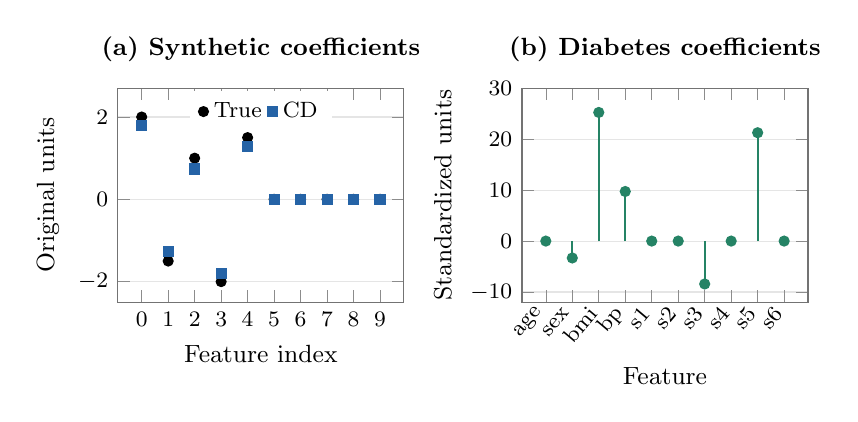
\begin{tikzpicture}
\begin{groupplot}[group style={group size=2 by 1,horizontal sep=1.5cm},width=.43\linewidth,height=4.3cm,
ymajorgrids=true,xtick={0,1,2,3,4,5,6,7,8,9}]
\nextgroupplot[title={(a) Synthetic coefficients},ylabel={Original units},xlabel={Feature index},ymin=-2.5,ymax=2.7,
legend style={at={(.5,.99)},anchor=north,legend columns=2}]
\addplot[black,only marks,mark=*,mark size=1.8pt] coordinates {(0,2.0) (1,-1.5) (2,1.0) (3,-2.0) (4,1.5) (5,0.0) (6,0.0) (7,0.0) (8,0.0) (9,0.0)};
\addlegendentry{True}
\addplot[lassoblue,only marks,mark=square*,mark size=1.8pt,error bars/.cd,y dir=both,y explicit] coordinates {(0,1.80100799) +- (0,0.0550045038) (1,-1.25970297) +- (0,0.035459667) (2,0.735873303) +- (0,0.0447481833) (3,-1.81046151) +- (0,0.0155839725) (4,1.28670574) +- (0,0.0187076477) (5,0) +- (0,0) (6,0) +- (0,0) (7,0) +- (0,0) (8,0) +- (0,0) (9,0) +- (0,0)};
\addlegendentry{CD}
\nextgroupplot[title={(b) Diabetes coefficients},ylabel={Standardized units},xlabel={Feature},
xticklabels={age,sex,bmi,bp,s1,s2,s3,s4,s5,s6},x tick label style={rotate=50,anchor=east},ymin=-12,ymax=30]
\addplot[lassogreen,ycomb,mark=*,mark size=1.6pt,thick] coordinates {(0,0) (1,-3.31495464) (2,25.2401022) (3,9.72941732) (4,-0) (5,-0) (6,-8.4190648) (7,0) (8,21.2607552) (9,0)};
\end{groupplot}\end{tikzpicture}
\caption{CD coefficients. Left: synthetic mean $\pm$ SD (original units); right: Diabetes (standardized units).}\label{fig:coefficients}\end{minipage}\end{center}

\subsection{Regularization effects}


\begin{center}\begin{minipage}{\linewidth}\captionsetup{type=table}\centering\small
\caption{Regularization study (CD).}\label{tab:penalty_results}
\begin{tabular*}{\linewidth}{@{\extracolsep{\fill}}crr@{}}\toprule
\textbf{$\lambda/\lambda_{\max}$} & \textbf{Test MSE} & \textbf{Nonzero}\\\midrule
\multicolumn{3}{@{}l}{\textit{Synthetic: three instances}}\\[2pt]
0.01 & $0.236\,{\pm}\,0.033$ & $22.3\,{\pm}\,3.5$\\
0.1 & $0.396\,{\pm}\,0.139$ & $5.0$\\
0.5 & $5.506\,{\pm}\,1.021$ & $4.3\,{\pm}\,0.6$\\
1 & $11.945\,{\pm}\,1.311$ & $0.0$\\
\midrule
\multicolumn{3}{@{}l}{\textit{Diabetes: fixed split}}\\[2pt]
0.01 & $2912.647$ & $8.0$\\
0.1 & $2966.937$ & $5.0$\\
0.5 & $3837.820$ & $2.0$\\
1 & $5893.048$ & $0.0$\\
\bottomrule\end{tabular*}\par\vspace{3pt}{\scriptsize $\mu\pm s$: three instances; nonzero: $|w_j|>10^{-6}$.}\end{minipage}\end{center}

\begin{center}\begin{minipage}{\linewidth}\captionsetup{type=figure}\centering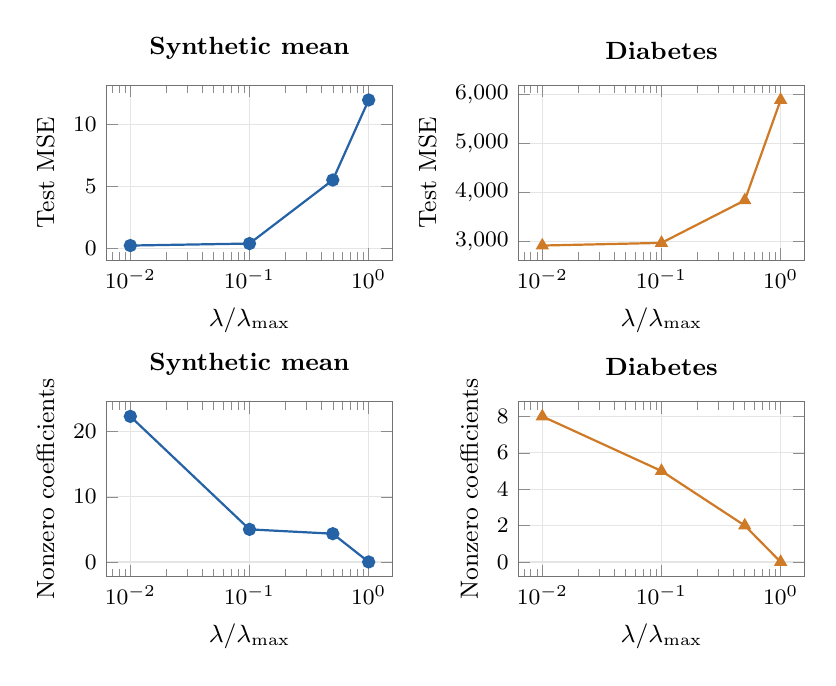
\begin{tikzpicture}
\begin{groupplot}[group style={group size=2 by 2,horizontal sep=1.6cm,vertical sep=1.8cm},width=.43\linewidth,height=3.8cm,xmode=log,
xlabel={$\lambda/\lambda_{\max}$},tick label style={font=\scriptsize},label style={font=\small},grid=major]
\nextgroupplot[title={Synthetic mean},ylabel={Test MSE}]
\addplot[lassoblue,mark=*,thick] coordinates {(0.01,0.235958863) (0.1,0.395982019) (0.5,5.50575318) (1.0,11.9445806)};
\nextgroupplot[title={Diabetes},ylabel={Test MSE}]
\addplot[lassoorange,mark=triangle*,thick] coordinates {(0.01,2912.6475) (0.1,2966.93661) (0.5,3837.82032) (1.0,5893.04764)};
\nextgroupplot[title={Synthetic mean},ylabel={Nonzero coefficients}]
\addplot[lassoblue,mark=*,thick] coordinates {(0.01,22.3333333) (0.1,5) (0.5,4.33333333) (1.0,0)};
\nextgroupplot[title={Diabetes},ylabel={Nonzero coefficients}]
\addplot[lassoorange,mark=triangle*,thick] coordinates {(0.01,8) (0.1,5) (0.5,2) (1.0,0)};
\end{groupplot}\end{tikzpicture}
\caption{Test MSE and selected variables versus penalty; synthetic means over three instances.}\label{fig:regularization}\end{minipage}\end{center}

Increasing the penalty reduced selected variables in these cases. For synthetic data, the mean count fell from 22.3 at ratio 0.01 to five at ratio 0.1, while mean test MSE rose from 0.2360 to 0.3960. The stronger penalty produced a smaller model without the lowest average prediction error. Individual errors were not strictly monotone: seed 1 had slightly lower MSE at 0.1 than at 0.01. At ratio 0.5, mean MSE rose to 5.5058, consistent with increased shrinkage bias.

For Diabetes, the selected count decreased from eight to five to two as the ratio increased from 0.01 to 0.1 to 0.5, and test MSE increased. At ratio 1, both datasets returned zero coefficients at initialization, as predicted by the optimality condition. Predictions then equal the training response mean. This fit--sparsity trade-off concerns the model and penalty, not superiority of CD as a predictor.

\section{Limitations and Conclusions}
Lasso's squared loss and separable $\ell_1$ penalty give three simple mechanisms: ISTA combines a gradient step with thresholding, FISTA adds extrapolation, and cyclic CD minimizes one coordinate with a maintained residual. Theory bounds objective error; experiments measure the cost of reaching a shared stationarity tolerance on the recorded synthetic and Diabetes training problems.

ISTA was fastest on the three synthetic instances, and CD was fastest on the fixed Diabetes split. Standard FISTA's stronger objective-error bound did not produce a time advantage under the common residual rule. Once converged, the solvers gave nearly identical objectives and predictions. Stronger penalties reduced selected variables but usually increased test error in the measured cases.

The experiment does not cover all feature correlations, high-dimensional regimes, or production solvers. Python loops, vectorized operations, and monitoring costs affect the results. Three synthetic instances give limited descriptive variation; timing repetitions are not independent data samples. A single real-data split cannot estimate uncertainty over splits. Test scores were not used to tune the penalty, and a small stationarity residual is not an objective-error certificate. The conclusions apply to the recorded datasets, preprocessing, implementations, and common stopping settings.


\subsection*{Generative AI assistance}
Generative AI tools assisted with literature organization, drafting, and experimental code. The reported experiments were executed locally, and citations were checked against primary sources.

\clearpage
\begingroup\small
\begin{thebibliography}{}
\setlength{\itemsep}{6pt}\setlength{\parskip}{0pt}
\bibitem[Beck and Teboulle(2009)]{beck2009}
Amir Beck and Marc Teboulle. 2009.
\href{https://doi.org/10.1137/080716542}{A fast iterative shrinkage-thresholding algorithm for linear inverse problems}.
\emph{SIAM Journal on Imaging Sciences}, 2(1):183--202.

\bibitem[Boyd and Vandenberghe(2004)]{boyd2004}
Stephen Boyd and Lieven Vandenberghe. 2004.
\href{https://web.stanford.edu/~boyd/cvxbook/}{Convex Optimization}.
Cambridge University Press.

\bibitem[Boyd et~al.(2011)Boyd, Parikh, Chu, Peleato, and Eckstein]{boyd2011}
Stephen Boyd, Neal Parikh, Eric Chu, Borja Peleato, and Jonathan Eckstein. 2011.
\href{https://doi.org/10.1561/2200000016}{Distributed optimization and statistical learning via the alternating direction method of multipliers}.
\emph{Foundations and Trends in Machine Learning}, 3(1):1--122.

\bibitem[Daubechies et~al.(2004)Daubechies, Defrise, and De~Mol]{daubechies2004}
Ingrid Daubechies, Michel Defrise, and Christine De Mol. 2004.
\href{https://doi.org/10.1002/cpa.20042}{An iterative thresholding algorithm for linear inverse problems with a sparsity constraint}.
\emph{Communications on Pure and Applied Mathematics}, 57(11):1413--1457.

\bibitem[Efron et~al.(2004)Efron, Hastie, Johnstone, and Tibshirani]{efron2004}
Bradley Efron, Trevor Hastie, Iain Johnstone, and Robert Tibshirani. 2004.
\href{https://doi.org/10.1214/009053604000000067}{Least angle regression}.
\emph{The Annals of Statistics}, 32(2):407--451.

\bibitem[Friedman et~al.(2010)Friedman, Hastie, and Tibshirani]{friedman2010}
Jerome H. Friedman, Trevor Hastie, and Rob Tibshirani. 2010.
\href{https://doi.org/10.18637/jss.v033.i01}{Regularization paths for generalized linear models via coordinate descent}.
\emph{Journal of Statistical Software}, 33(1):1--22.

\bibitem[Hoerl and Kennard(1970)]{hoerl1970}
Arthur E. Hoerl and Robert W. Kennard. 1970.
\href{https://doi.org/10.1080/00401706.1970.10488634}{Ridge regression: Biased estimation for nonorthogonal problems}.
\emph{Technometrics}, 12(1):55--67.

\bibitem[Kim et~al.(2007)Kim, Koh, Lustig, Boyd, and Gorinevsky]{kim2007}
Seung-Jean Kim, Kwangmoo Koh, Michael Lustig, Stephen Boyd, and Dimitry Gorinevsky. 2007.
\href{https://doi.org/10.1109/JSTSP.2007.910971}{An interior-point method for large-scale $\ell_1$-regularized least squares}.
\emph{IEEE Journal on Selected Topics in Signal Processing}, 1(4):606--617.

\bibitem[Ndiaye et~al.(2017)Ndiaye, Fercoq, Gramfort, and Salmon]{ndiaye2017}
Eugene Ndiaye, Olivier Fercoq, Alexandre Gramfort, and Joseph Salmon. 2017.
\href{https://jmlr.org/papers/v18/16-577.html}{Gap Safe screening rules for sparsity enforcing penalties}.
\emph{Journal of Machine Learning Research}, 18(128):1--33.

\bibitem[O'Donoghue and Cand\`es(2015)]{odonoghue2015}
Brendan O'Donoghue and Emmanuel Cand\`es. 2015.
\href{https://doi.org/10.1007/s10208-013-9150-3}{Adaptive restart for accelerated gradient schemes}.
\emph{Foundations of Computational Mathematics}, 15:715--732.

\bibitem[Parikh and Boyd(2014)]{parikh2014}
Neal Parikh and Stephen Boyd. 2014.
\href{https://doi.org/10.1561/2400000003}{Proximal algorithms}.
\emph{Foundations and Trends in Optimization}, 1(3).

\bibitem[scikit-learn developers(2026)]{sklearn_data}
scikit-learn developers.
\href{https://scikit-learn.org/stable/modules/generated/sklearn.datasets.load_diabetes.html}{Diabetes dataset}
and \href{https://scikit-learn.org/stable/modules/generated/sklearn.linear_model.Lasso.html}{Lasso}.
Documentation, release 1.9.1; accessed 5 October 2026.

\bibitem[Tibshirani(1996)]{tibshirani1996}
Robert Tibshirani. 1996.
\href{https://doi.org/10.1111/j.2517-6161.1996.tb02080.x}{Regression shrinkage and selection via the lasso}.
\emph{Journal of the Royal Statistical Society: Series B (Methodological)}, 58(1):267--288.

\bibitem[Tibshirani(2013)]{tibshirani2013}
Ryan J. Tibshirani. 2013.
\href{https://doi.org/10.1214/13-EJS815}{The lasso problem and uniqueness}.
\emph{Electronic Journal of Statistics}, 7:1456--1490.

\bibitem[Tseng(2001)]{tseng2001}
Paul Tseng. 2001.
\href{https://doi.org/10.1023/A:1017501703105}{Convergence of a block coordinate descent method for nondifferentiable minimization}.
\emph{Journal of Optimization Theory and Applications}, 109(3):475--494.

\bibitem[Wright(2015)]{wright2015}
Stephen J. Wright. 2015.
\href{https://doi.org/10.1007/s10107-015-0892-3}{Coordinate descent algorithms}.
\emph{Mathematical Programming}, 151(1):3--34.

\bibitem[Wu and Lange(2008)]{wu2008}
Tong Tong Wu and Kenneth Lange. 2008.
\href{https://doi.org/10.1214/07-AOAS147}{Coordinate descent algorithms for lasso penalized regression}.
\emph{The Annals of Applied Statistics}, 2(1):224--244.

\bibitem[Zhao and Yu(2006)]{zhao2006}
Peng Zhao and Bin Yu. 2006.
\href{https://jmlr.org/papers/v7/zhao06a.html}{On model selection consistency of Lasso}.
\emph{Journal of Machine Learning Research}, 7(90):2541--2563.

\bibitem[Zou(2006)]{zou2006}
Hui Zou. 2006.
\href{https://doi.org/10.1198/016214506000000735}{The adaptive lasso and its oracle properties}.
\emph{Journal of the American Statistical Association}, 101(476):1418--1429.

\bibitem[Zou and Hastie(2005)]{zou2005}
Hui Zou and Trevor Hastie. 2005.
\href{https://doi.org/10.1111/j.1467-9868.2005.00503.x}{Regularization and variable selection via the elastic net}.
\emph{Journal of the Royal Statistical Society: Series B (Statistical Methodology)}, 67(2):301--320.

\end{thebibliography}
\endgroup
\end{document}
